% MySubmissionOnlineSupplementAtJournMathMusic.tex
% v1.1 prepared by Thomas Fiore
% Thomas Fiore retains the copyright for the content of this template.

%%%%%%%%%%%%%%%%%% NOTE TO AUTHORS%%%%%%%%%%%%%
% Please use this template to prepare your submission Online Supplement PDF.
% Do not include your name in the file-name because the file-name displays in the compiled PDF at the top of every page. Your name should not be included there in order to guarantee double-blind reviewing.
% After reading the pre-compiled pdf file, rename this LaTeX file, delete the relevant passages, and fill in the blanks according to the comment lines in this file.
% This file is the quick-start LaTeX template for your Online Supplement.
% More detailed instructions are in the main file and in the tMAMguide.pdf file if needed.
% IMPORTANT: The Online Supplement is not edited by the production department. If the main article is accepted,
% the Online Supplement will be posted directly online, so it must be ``camera ready'' and in final form.
% Use PDFLaTex and BibTex to compile. PDFLaTeX is necessary to create the hyperlinks.
%%%%%%%%%%%%%%%%%%%%%%%%%%%%%%%%%%%%%%%%%%%%%%%%%

\documentclass[suppldata]{tMAM2e}% Do not change this line. The option ``[suppldata]'' is turned on to make the
%Online Supplement format. The style file tMAM2e must be in your working directory. This style file is the same style file
%as the main file.

\usepackage{epstopdf}% To incorporate .eps illustrations using PDFLaTeX, etc.
\usepackage[bookmarksnumbered,colorlinks,bookmarks,citecolor=blue,linkcolor=blue,urlcolor=blue,breaklinks,linktocpage]{hyperref}% To create hyperlinks using PDFLaTeX, etc.
\usepackage[all]{hypcap}% This turns on the hyperlinks for \label{} and \ref{}, and others.
\usepackage{subfigure}% Support for small, `sub' figures and tables
\usepackage{graphicx}

%%% DEFINITIONS


\newcommand{\RR}{\mathbb{R}}
\newcommand{\vect}[1]{\mathbf{#1}}
\newcommand{\vectm}{\vect m}
\newcommand{\vx}{\vect x}
\newcommand{\vy}{\vect y}
\newcommand{\vp}{\vect p}
\newcommand{\vq}{\vect q}
\newcommand{\vr}{\vect r}
\newcommand{\vs}{\vect s}
\newcommand{\vc}{\vect c}
\newcommand{\ir}{\textsc{ir}}

%%%%%%%%%%%%%%%

\theoremstyle{plain}
\newtheorem{theorem}{Theorem}[section]
\newtheorem{corollary}[theorem]{Corollary}
\newtheorem{lemma}[theorem]{Lemma}
\newtheorem{proposition}[theorem]{Proposition}

\theoremstyle{definition}
\newtheorem{definition}[theorem]{Definition}

\theoremstyle{remark}
\newtheorem{remark}[theorem]{Remark}
\newtheorem{example}[theorem]{Example}

\begin{document}

% If accepted, the following lines must be replaced by the actual data.
\jvol{{\bf INSERT NONBOLD}} \jnum{{\bf INSERT NONBOLD KEEP COMMA},} \jyear{{\bf INSERT YEAR NONBOLD}}
\doi{\hspace{-.08in}\href{INSERT DOI LINK FROM PUBLISHER TWICE}{{\color{black}INSERT DOI LINK FROM PUBLISHER TWICE}}}

% The title of the Online Supplement is: Online Supplement to ``Main article title''
% Note the capitalization: only the first word and proper nouns are capitalized..
\title{Online Supplement to ``Rhythmic segment analysis: Conceptualizing, visualizing, and measuring rhythmic data''}

% The author formatting should be exactly as in your main file. See the comments there.

\author{
% \name{Bas Cornelissen\textsuperscript{a}$^{\ast}$\thanks{$^\ast$Corresponding author. Email: mail@bascornelissen.nl}}
%
% @EDITOR: I hope you forgive me for adding a linebreak after the institute; improves the balance
%
% \affil{\textsuperscript{a}Institute for Logic, Language and Computation,\\
% University of Amsterdam, Amsterdam, The~Netherlands}
%leave blank for production:
\received{}
}

\maketitle

% \noindent Please note: the production department does not work on Online Supplements so your Online Supplement must be camera ready after acceptance, and will be posted directly online. The data in the upper left corner will be provided to you after acceptance, for inclusion before posting.

\begin{abstract}
This Online Supplement contains (1) a more formal development of the ideas presented in the paper, (2) additional synthetic datasets complementing the section `Visualization' in the paper, and (3) additional analyses and figures for the case study on Cuban salsa and son.
\end{abstract}


% Keywords
\begin{keywords}
rhythmic segment analysis; rhythm ratio; isochrony; anisochrony; nPVI; quantal data
\end{keywords}

% AMS MSC and MCM CCS
\begin{classcode}\textit{2020 Mathematics Subject Classification}: 00A65 \\
\textit{2012 Computing Classification Scheme}: applied computing
\end{classcode}


%%%%%%%%%%%%%%%%%%%%%%%%%%%%%%%%%%%%%%%%%%%%%%%%%%%%%%%%%%%%%%%%%%%%%%%%%%%%%%%%%%%%%%%%%%%%%



\section{Mathematical framework}


\subsection{Segments and patterns}

Consider a dataset $\{t_1, \dots, t_{K+1}\}$ of distinct events ordered in time, and let $i_k = t_{k+1}-t_k$ denote the time intervals between them.
We may in practice assume that intervals are strictly positive, but formally we can allow for zero intervals.
Any sequence of $n$ consecutive (and nonnegative) intervals $\vx = (i_k, \dots, i_{k+n})$ will be called a \emph{segment} of length $n$.
We will use the $L_1$-norm,
\begin{align}
  \|\vx\|_1 = |x_1| + \dots + |x_n|,
\end{align}
so that the norm or length of a segment equals its duration.
Accordingly, we measure the distance between two segments $\vx$ and $\vy$ as
\begin{align}
  \|x-y\|_1 = \sum_{i=1}^n |x_i-y_i|
\end{align}
This distance is known as the \emph{taxicab} distance, but we will refer to it as the \emph{segment distance} $d_s$.


\begin{definition}
  The \emph{segment space} $\mathcal{S}^n$, for $n\ge 2$, consists of non-zero and nonnegative vectors $\RR_{\ge 0}^n \setminus \{0\}$ equipped with the $L_1$-norm $\|\cdot\|_1$ and the \emph{segment distance} $d_s(x, y) = \|x-y\|_1$.
\end{definition}

Two segments $(0.1, 0.2, 0.1)$ and $(2, 4, 2)$ can have a different duration, but still form the same rhythmical \emph{pattern}.
That pattern can be expressed equivalently by either the \emph{ratios} $1 : 2 : 1$ or by a normalized vector $(0.25, 0.5, 0.25)$ containing the relative durations of all intervals.
The $(n-1)$-dimensional \emph{simplex} $\Delta^{n-1}$ is exactly the space of nonnegative and normalized vectors:
\begin{align}
  \Delta^{n-1}
  = \{ \vx \in \RR_{\ge 0}^n: x_1 + \dots + x_n = 1\}.
\end{align}
We will equip the simplex with the \emph{total variation distance}, which is half the taxicab distance, and will refer to it as the \emph{pattern distance} $d_p$.
This distance is normalized, so that the total variation distance between any two corners of the simplex is 1.\footnote{%
  Two corners $\vp$ and $\vq$ have all-zero coordinates, except for a single 1 in different places. 
Therefore, $\tfrac{1}{2}\|\vp-\vq\|_1 = \tfrac{1}{2} (|0-1| + |1 - 0|) = 1$.
}

\begin{definition} For $n\ge 2$, the \emph{pattern space} $\mathcal{P}^n$ is the simplex $\Delta^{n-1}$ equipped with the \emph{total variation distance} $d_p(\vp, \vq) = \tfrac{1}{2}\|\vp - \vq\|_1$.
\end{definition}

\subsection{Pattern-duration space}

Every segment $\vx$ can be uniquely decomposed into a pattern $\vp = \vx / \|\vx\|_1$ and a duration $d = \|\vx\|_1$.
Figure \ref{fig:coordinate-transform} illustrates that you can think of this as a coordinate transform to the point $(p, d)$ in the \emph{pattern-duration space} $\Delta^{n-1} \times \RR_{>0}$.
Conversely, multiplying a pattern by its duration moves back to the original space.
Formally, the function $\Phi$ takes care of all this:
\begin{align}
  \Phi(\vx) = \left(\frac{\vx}{\|\vx\|_1}, \;\; \|\vx\|_1\right), \qquad
  \Phi^{-1}(\vp, d) = d\cdot \vp
\end{align}

\begin{figure}
  \centering
  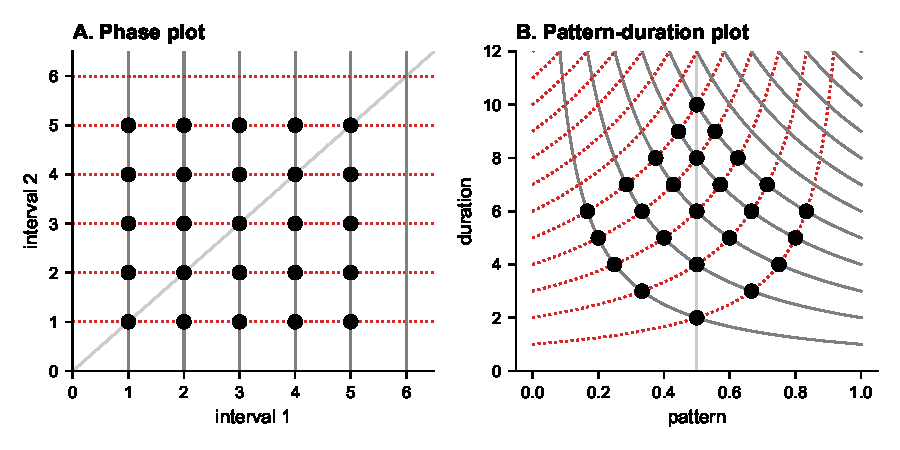
\includegraphics[width=.8\textwidth]{../../figures/coordinate-transform.pdf}
  \caption{A coordinate transform turns the phase space into a pattern-duration space. 
\label{fig:coordinate-transform}}
\end{figure}

Geometrically, the pattern-duration decomposition described here can be understood as the \emph{taxicab equivalent of spherical coordinates}.
A radial-angular decomposition (the more general term for spherical coordinates) locates a point using a radius and a direction. 
The direction is specified by several angles that determine a point on the unit ball.
Since segments are non-negative sequences, we are only concerned with the non-negative part of $\RR^n$ (i.e. the non-negative orthant).
In taxicab geometry, the unit ball on that part of the space coincides precisely with a simplex.
And so a pattern—a point on the simplex—specifies a direction as a point on the unit ball, while the radius under the $L_1$ norm equals the duration of a segment.
In short, the pattern gives a direction and the duration is the radius.


Knowing how to move between segment space and pattern-duration space, we can pull the taxicab distance from the segment space to define the \emph{pattern-duration distance $d_{pd}$} on the pattern-duration space:
\begin{align}
  d_{pd}\Big((\vp, d), (\vq, e)\Big)
  = \|d\vp - e\vq\|_1
\end{align}
This distance plays well with the underlying distances. 
If two pattern-duration pairs share their patterns but not their durations, their distance is the absolute duration difference:
\begin{align}
  % d_{pd}\Big((\vp, d), (\vp, e)\Big)
  \|d\vp - e\vp\|_1
  % = \|d\vp - e\vp\|_1 
  = |d-e| \cdot \|\vp\|_1
  = |d-e|,
\end{align}
where we use that patterns are normalized, so that $\|\vp\|_1=1$.
Conversely, if two pairs have the same duration $e$, but different patterns, their distance reduces to the distance between the patterns multiplied by twice the duration:
\begin{align}
  % d_{pd}\Big((\vp, e), (\vq, e)\Big)
  \|d \vp - d \vq\|_1
  = d \cdot \|\vp - \vq\|_1
  = 2d \cdot d_p(\vp, \vq).
\end{align}
The factor two compensates for the fact that the total variation distance is half the taxicab distance.


\subsection{Quantal data}

If musical rhythm adheres to a grid, there is a smallest interval, a 'time quantum', of which all intervals are (integer) multiples. 
The interval distributions may accordingly show clustering around those quantum multiples, as in Figure~\ref{fig:interval-distributions}A, B, and F. 
It motivates the following definition.

\begin{definition}
  A rhythmic dataset is \emph{quantal} when the interval distribution is a mixture of clusters close to integer multiples of a fixed \emph{quantum}.
\end{definition}

In a quantal dataset, individual intervals will also approximate quantum multiples, but I choose not to define quantal data in this way.
Firstly, the motivating model is one where an observed interval is a noisy rendition of a latent interval category.
The structure of interest is the latent structure, not the noise, and so it seems more appropriate to define the concept in terms of the cluster structure.
Secondly, if we call a dataset quantal when its intervals approximate quantum multiples, then any dataset will become quantal by choosing the quantum small enough.
Defining quantal data in terms of clusters does not resolve this entirely.
Indeed, the definition remains informal until one specifies (1) what constitutes narrow and well-separated clustering, (2) a maximum distance between a cluster and the closest quantum multiple, and (3) a lower bound for the quantum relative to the shortest interval cluster.
% For example $\tfrac{1}{4}q$ 
% (e.g. one order of magnitude, so $q > \tfrac{m}{10}$ where $m$ is the smallest mode).



\subsection{Integer ratios}

The notion of quantal data is closely related to the presence of integer-ratio rhythms—but what does the latter even mean?
In terms of segments and patterns, there are two possible readings: (1) that \emph{patterns} cluster around integer ratios or (2) that \emph{segments} cluster around integer ratios.
The first reading seems to be the default and is consistent with the use of ratio plots.
I would, however, argue for the second reading.
To explain why, I will define the two readings more explicitly, yet without completely formalizing them.
I will assume that clusters are narrow, separated regions of high-density in the distribution;
segments with only integer entries will be called \emph{integer segments}; and patterns of integer segments are \emph{integer-ratio patterns}. 
The first reading amounts to the following.


\begin{definition}
  Rhythmic data has \emph{integer-ratio pattern clusters} if the pattern distribution is a mixture of clusters close to integer-ratio patterns.
\end{definition}

This means that a ratio plot should show clear clustering around integer-ratio patterns.
But in the main text, I pointed to a problem: distinct \emph{segment} clusters can create overlapping pattern clusters.
Figure \ref{fig:flat-ratio-plot} illustrates this point. 
It shows a repeated rhythm that is designed to traverse very similar patterns, resulting in an almost flat ratio plot, or in any case one that underestimates the number of segment clusters.
And for that reason, I would argue for defining the presence of integer-ratio rhythms in terms of the segments, not the patterns.

\begin{figure}
  \centering%
  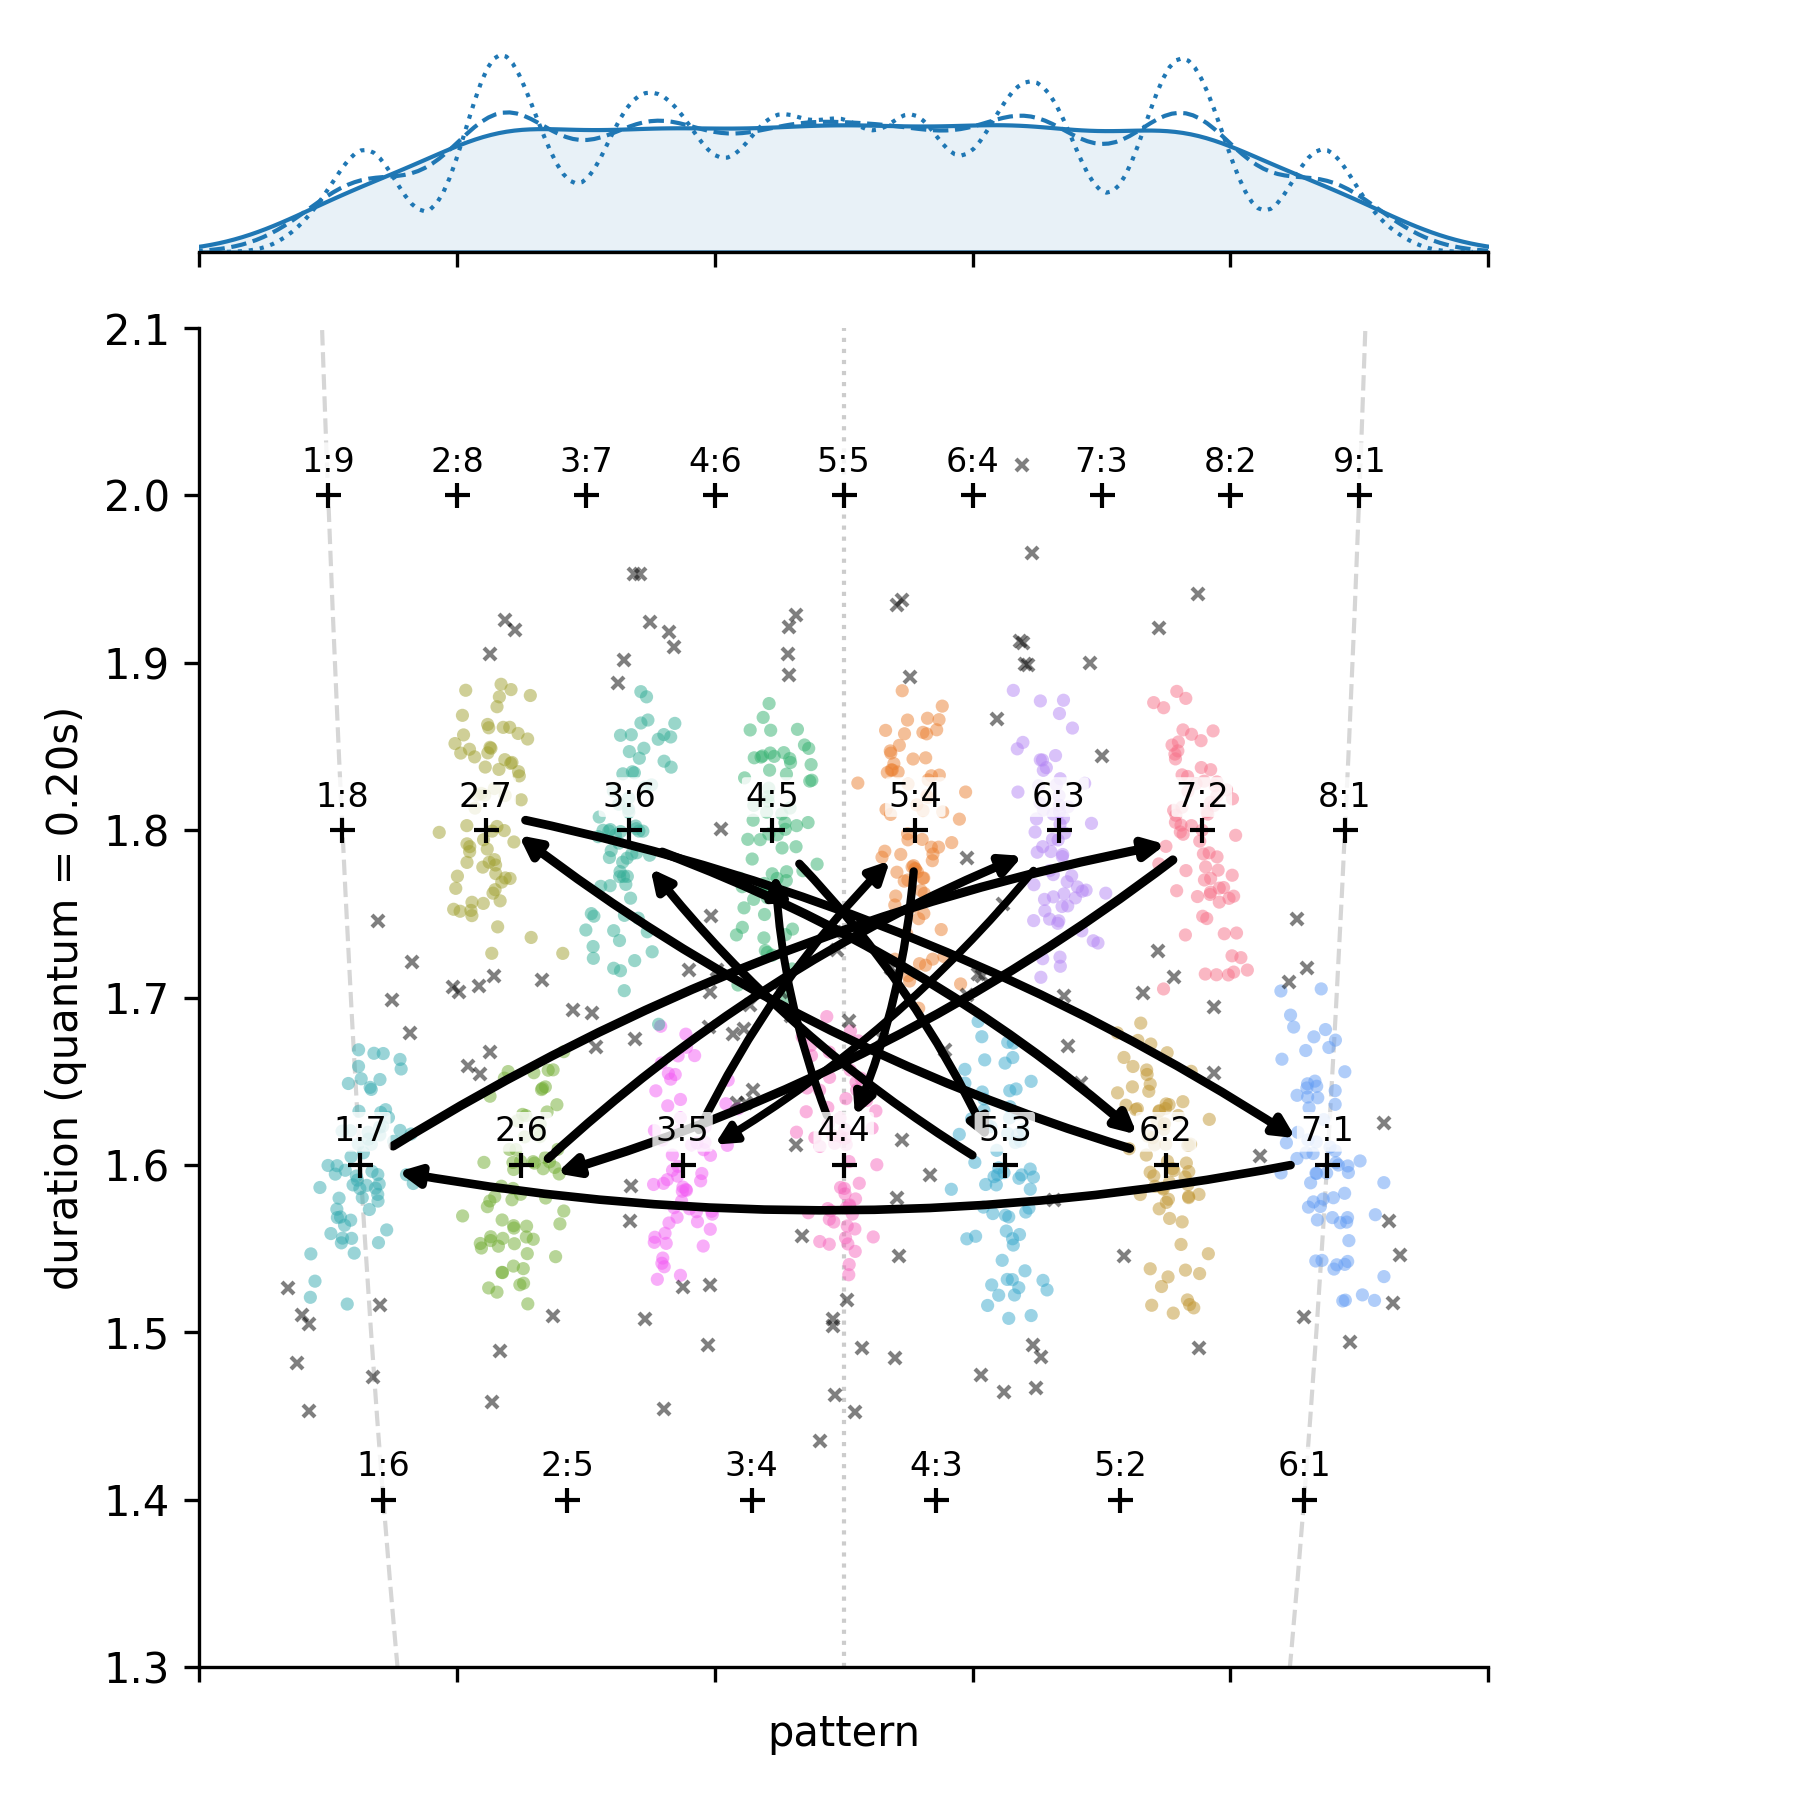
\includegraphics[width=.7\textwidth]{../../figures/flat-ratio-plot.png}
  \caption{%
    Overlapping segment clusters can distort the number of rhythmic categories in ratio plots. 
    A repeated rhythm traverses proximate ratios such as 2:7 and 2:6. 
    When projected on the horizontal axes, some of these clusters disappear (top). 
    Kernel density plots are sensitive to the bandwidth parameter; the dotted and dashed lines show kernel density estimates with ever smaller bandwidths.
    \label{fig:flat-ratio-plot}
  }
\end{figure}


\begin{definition}
  Rhythmic data has \emph{integer-ratio segment clusters} if there is a fixed number $q$ such that segment distribution is a mixture of clusters, each close to $q \cdot \vectm$ for some integer segment $\vectm$.
\end{definition}

In pattern-duration space, integer-ratio segment clusters are clusters with integer-ratio patterns and whose durations are all integer multiples of the same interval $q$.
As may be clear by now, this is very closely tied to the concept of quantality: they are equivalent.


\begin{theorem}
  A dataset has integer-ratio segment clusters if and only if it is quantal.
\end{theorem}

\begin{proof}[Proof sketch]
  Suppose a dataset has integer-ratio segment clusters, so that each cluster is close to $q \vectm$ for some integer segment $\vectm$.
  Projecting on any coordinate gives the interval distribution, which will have a cluster close to the corresponding quantum multiple. 
  This implies the dataset is quantal.
  Conversely, if the dataset is quantal all intervals are of the form $q m + \delta$ for some integer $m$ and a small $\delta$. 
  That implies that each segment is close to $q \vectm$ for some integer segment $\vectm$ and we find integer-ratio segment clustering.
\end{proof}

This suggests that the presence of integer ratios and quantality are two sides of the same coin, which means that one can replace questions about integer ratios with questions about quantality.

\subsection{Anisochrony and the nPVI}

In this section we define a measure of \emph{anisochrony} and show how it relates to the normalized pairwise variability index (nPVI).
First, some notation and properties.
Let the \emph{centroid} of a simplex be written as $\vc = (\tfrac{1}{n}, \dots, \tfrac{1}{n})$.
The distance from any corner $\vp$ to the centroid is $(n-1)/n$. 
To see this, note that $\vp$ contains only zeros and a single one. 
It follows that the distance to the centroid is
\begin{align}
  \tfrac{1}{2}\Big((n-1) \cdot |0 - \tfrac{1}{n}| +
  |1-\tfrac{1}{n}|\Big)
  = \tfrac{1}{2}\Big(\frac{n-1}{n} + \frac{n-1}{n}\Big)
  = \frac{n-1}{n}.
\end{align}
We can use this to define the anisochrony of a pattern as the normalized distance from isochrony (i.e. the centroid). 
Although we define it for patterns, we can naturally extend the definition to segments.


\begin{definition}
  The \emph{anisochrony} of a pattern $\vp$ is the normalized distance from isochrony, represented by the centroid $\vc$:
  \begin{align}
    \alpha(\vp)
    \; := \; \frac{n}{n-1} \cdot d_p(\vp, \vc)
    \; = \; \frac{n}{2(n-1)} \sum_{i=1}^n |p_i - \tfrac{1}{n}|
  \end{align}
  The anisochrony of a segment $\vx$ is the anisochrony of its pattern $\vx / \|\vx\|_1$.
\end{definition}



For patterns of length $n=2$ this definition can be simplified.
To that end, note that when two positive numbers $a$ and $b$ sum to one, we have
\begin{align}
  |a-\tfrac{1}{2}| = |b-\tfrac{1}{2}|
  \qquad \text{and} \qquad
  |a-b|
  = |a-\tfrac{1}{2}| + |b-\tfrac{1}{2}|.
\end{align}
The first property follows directly from $a=b-1$. 
For the second one, write
$|a-b|
  = |a-(1-a)|
  = |2a-1|
  = 2|a-\tfrac{1}{2}|
  = |a-\tfrac{1}{2}| + |b-\tfrac{1}{2}|
$,
using the first property in the last step.
The second equality proves the following result, when noting that the normalizing constant in the definition of anisochrony disappears when $n=2$.

\begin{theorem}\label{thm:2-anisochrony}
  The anisochrony of a pattern of length 2 is $\alpha((p_1, p_2)) = |p_1 - p_2|$.
\end{theorem}

Now we can turn to the normalized pairwise variability index for a sequence of intervals $(i_1, \dots, i_K)$, which is defined as
\begin{align}
  \text{nPVI}
  = \frac{200}{K-1} \sum_{k=1}^{K-1}
  \Big| \frac{i_k - i_{k+1}}{i_k + i_{k+1}} \Big|.
\end{align}
The previous result almost immediately shows that the nPVI is proportional to the average anisochrony.

\begin{theorem}
  The nPVI is 200 times the average anisochrony of length-2 segments.
\end{theorem}
\begin{proof}
  Consider intervals $i_1, \dots i_K$.
  Theorem \ref{thm:2-anisochrony} shows that the anisochrony of the $k$-th pattern $\vp_k$ is
  \begin{align}
    \alpha(\vp_k)
    = \Big|
    \frac{i_k - i_{k+1}}{i_k+i_{k+1}}
    \Big|,
    \quad \text{where}\;
    \vp_k = \Big(\frac{i_k}{i_k+i_{k+1}}, \;\frac{i_{k+1}}{i_k+i_{k+1}}\Big),
  \end{align}
  which is a summand in the definition of the nPVI.
  It follows that the average anisochrony $\tfrac{1}{K-1}\sum_k \alpha(\vp_k)$
  equals $\tfrac{1}{200} \times \text{nPVI}$.
\end{proof}


\section{Synthetic data}

The main text compares visualizations of three types of synthetic rhythmic data. 
These supplements include some additional plots for three more synthetic datasets.
Interval distributions of all datasets are shown in Figure~\ref{fig:interval-distributions}.

\begin{itemize}
  \item \textbf{Uniform quantal}. 
  Integers $k$ were sampled uniformly between 1 and 11. 
  Gaussian noise $\epsilon \sim \text{Normal}(0, 0.1)$ was added, and the result scaled by a quantum of $0.2$ to get intervals $i = 0.2 (k + \epsilon)$.
  
  \item \textbf{Geometric quantal}. 
  Integers $k$ were sampled from a geometric distribution with parameter $p=0.5$ to favour small integers. 
  This results in intervals $i=0.2(k+\epsilon)$ with $\epsilon \sim \text{Normal}(0, 0.1)$ as before.
  
  \item \textbf{Uniform}. 
  Intervals were sampled uniformly between 0.2 and 2.
  
  \item \textbf{Normal}. 
  Intervals were sampled from a $\text{Normal}(1, 0.5)$ distribution, truncated at 0, so only positive samples were retained.
  
  \item \textbf{Isochrony}. 
  Idem, but with smaller variance: using $\text{Normal}(0, 0.05)$.
  
  \item \textbf{Repeated}. 
  The template $(1, 1, 2, 1, 2, 2, 1, 2, 1, 1, 2, 1, 2, 2, 1, 2, 3, 3, 2, 4)$ of integer intervals was repeated (see Figure~\ref{fig:repeated-rhythm}), Gaussian noise $\epsilon \sim \text{Normal}(0, 0.1)$ was added as before, and the result was scaled by a quantum of 0.5 to get intervals $i=0.5(k + \epsilon)$.
\end{itemize}

\begin{figure}[h!]
  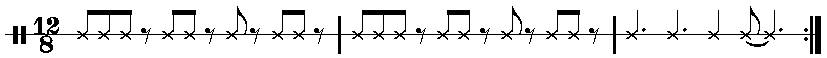
\includegraphics[width=\textwidth]{../../scores/repeated-rhythm.pdf}
  \caption{
    The repeated dataset consists of repetitions of this rhythm, with some noise added. 
    The reader may recognize the first two bars as the backbone of Steve Reich’s \emph{Clapping Music}.
    \label{fig:repeated-rhythm}
  }
\end{figure}


\begin{figure}[h]
  \centering
  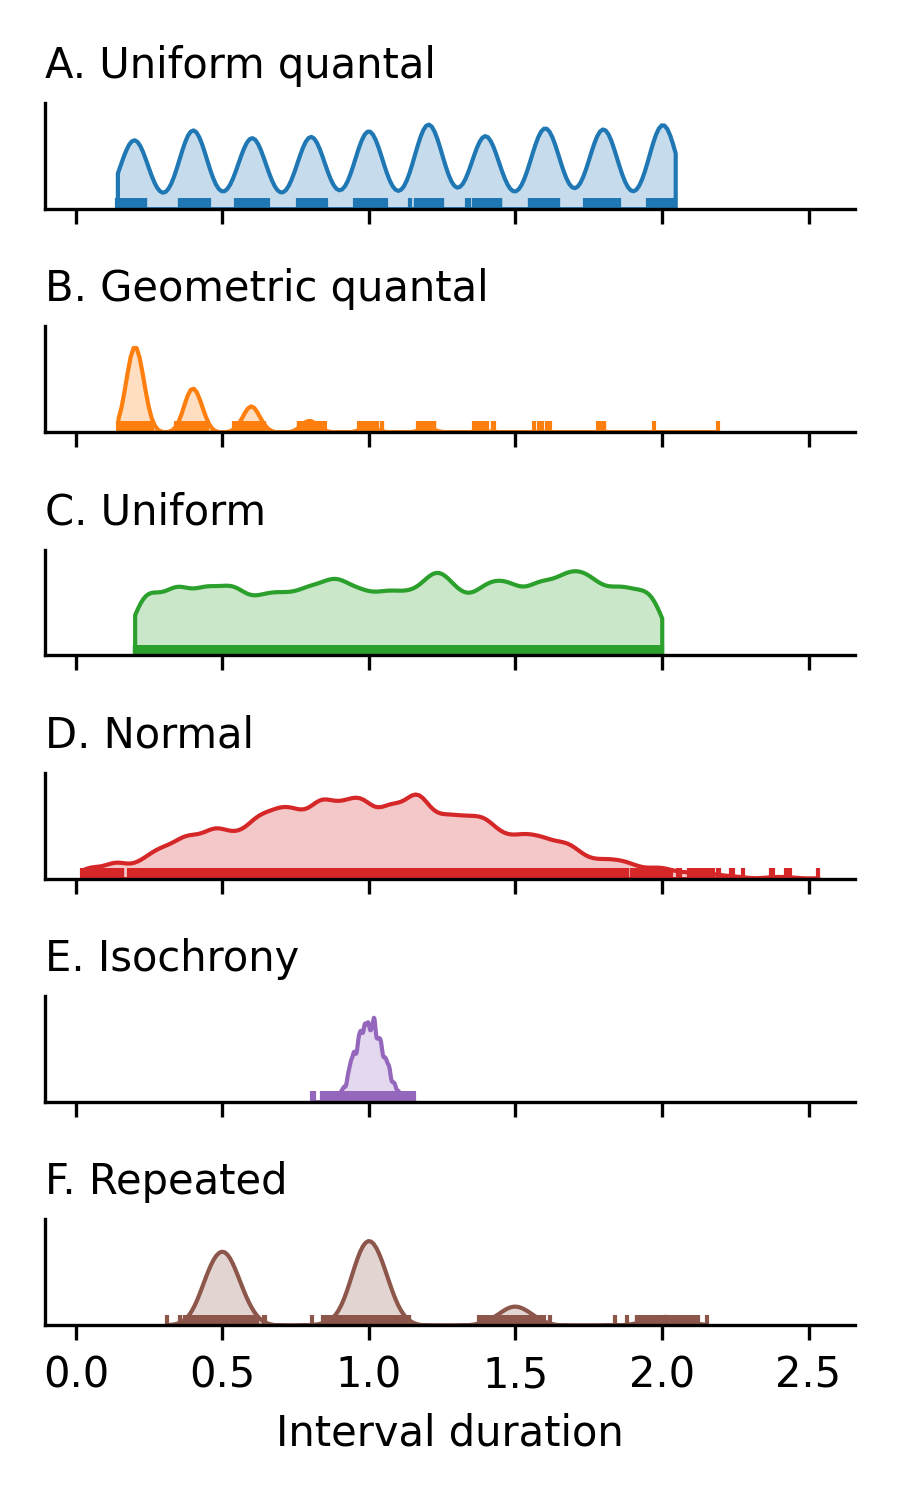
\includegraphics[width=.3\textwidth]{../../figures/synthetic-intervals-distributions.png}
  \caption{%
    Interval distributions for all synthetic datasets.
    \label{fig:interval-distributions}%
  }
\end{figure}



\begin{figure}[h!]
  \centering
  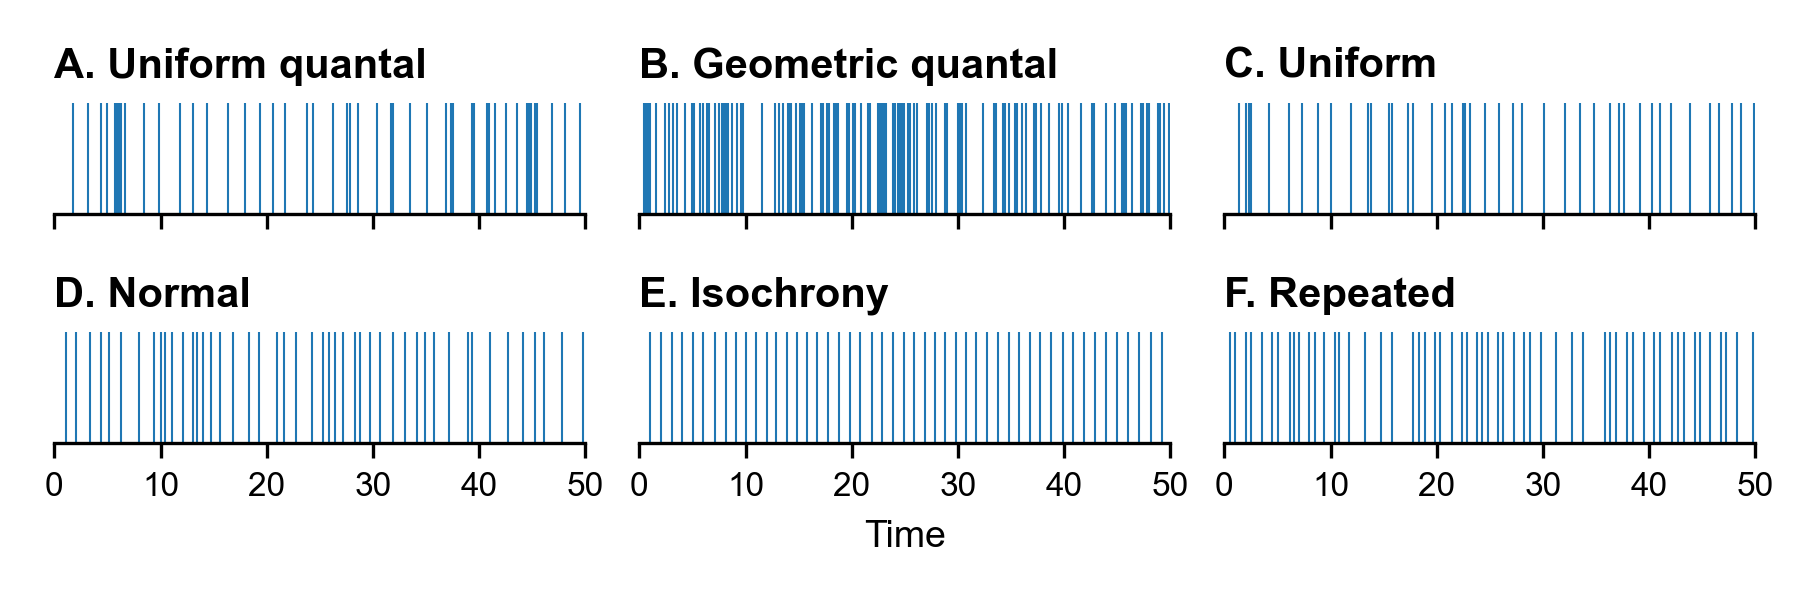
\includegraphics[width=.7\textwidth]{../../figures/plot-types/event-plots.png}
  \caption{%
    Event plots of synthetic rhythmic data in which each event is marked with a vertical line.
    \label{fig:event-plots}%
  }
\end{figure}


\begin{figure}[h!]\centering
  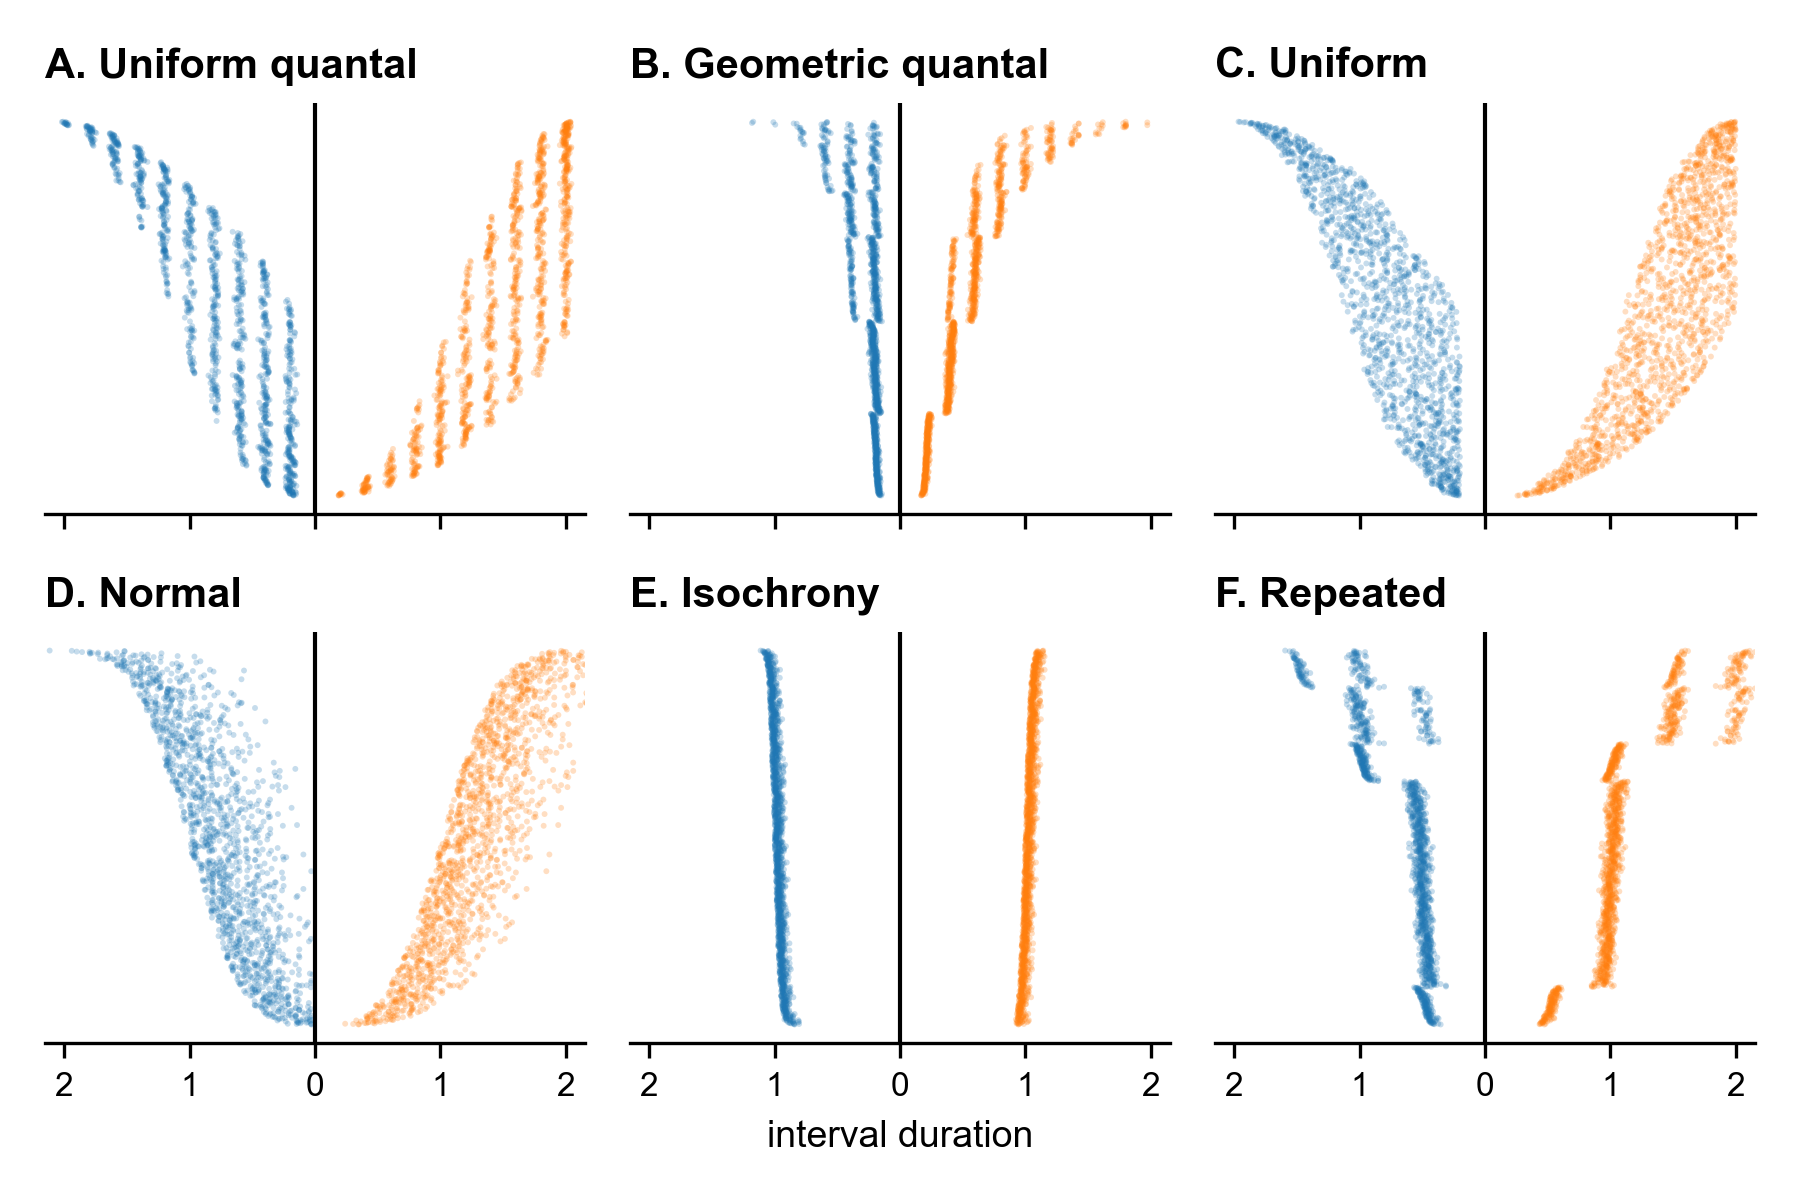
\includegraphics[width=.7\textwidth]{../../figures/plot-types/raster-plots.png}
  \caption{%
    Raster plots for synthetic rhythmic data. 
    Every segment is plotted using two points: the shorter of the two intervals on the left in blue and the longer one on the right in orange.
    Segments are sorted vertically by their duration, with shorter segments at the bottom.
    \label{fig:raster-plots}%
  }
\end{figure}

\begin{figure}[h!]\centering
  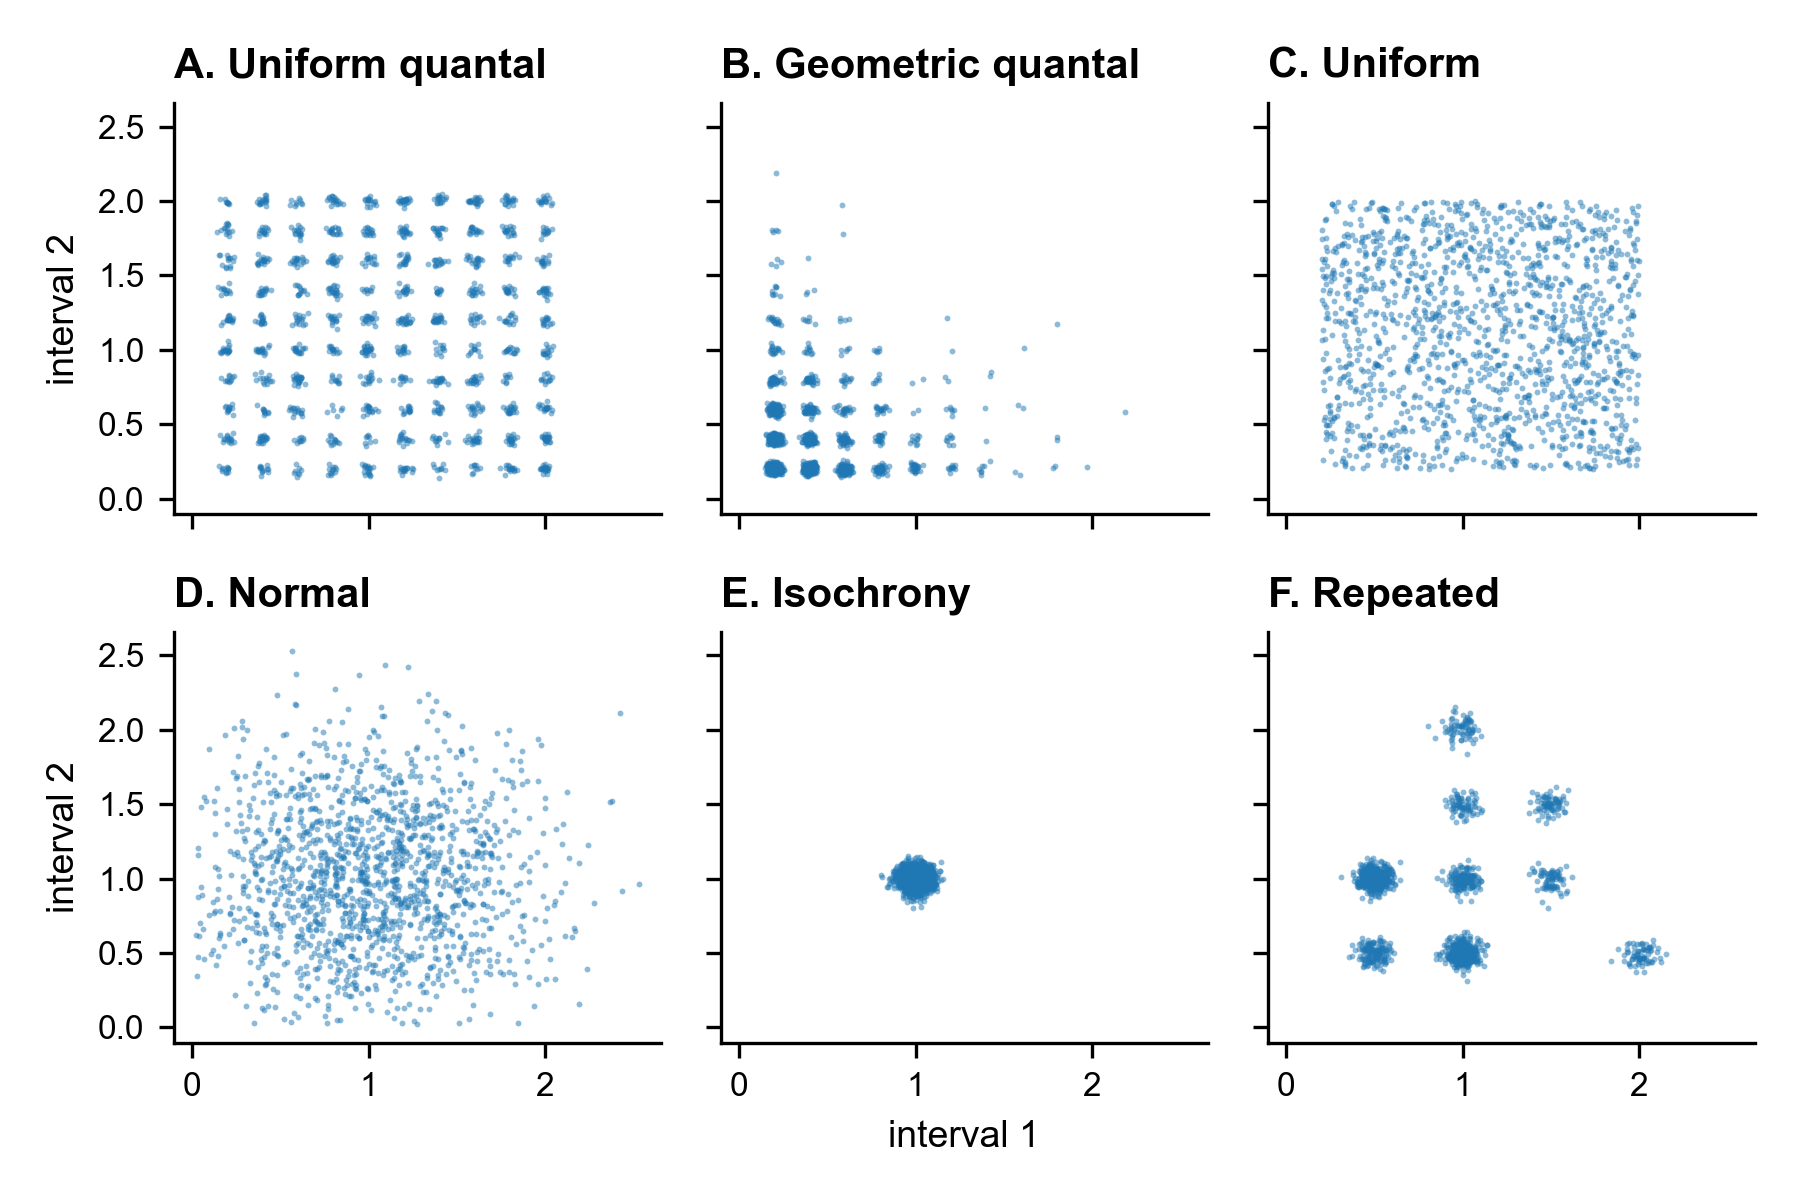
\includegraphics[width=.7\textwidth]{../../figures/plot-types/phase-plots-scatter.png}
  \caption{
    Scatter phase plots of synthetic rhythmic data where each segment is shown as a point, with the duration of the first interval horizontally and the duration of the second interval vertically.
    \label{fig:phase-plot-scatter}%
  }
\end{figure}

\begin{figure}[h!]\centering
  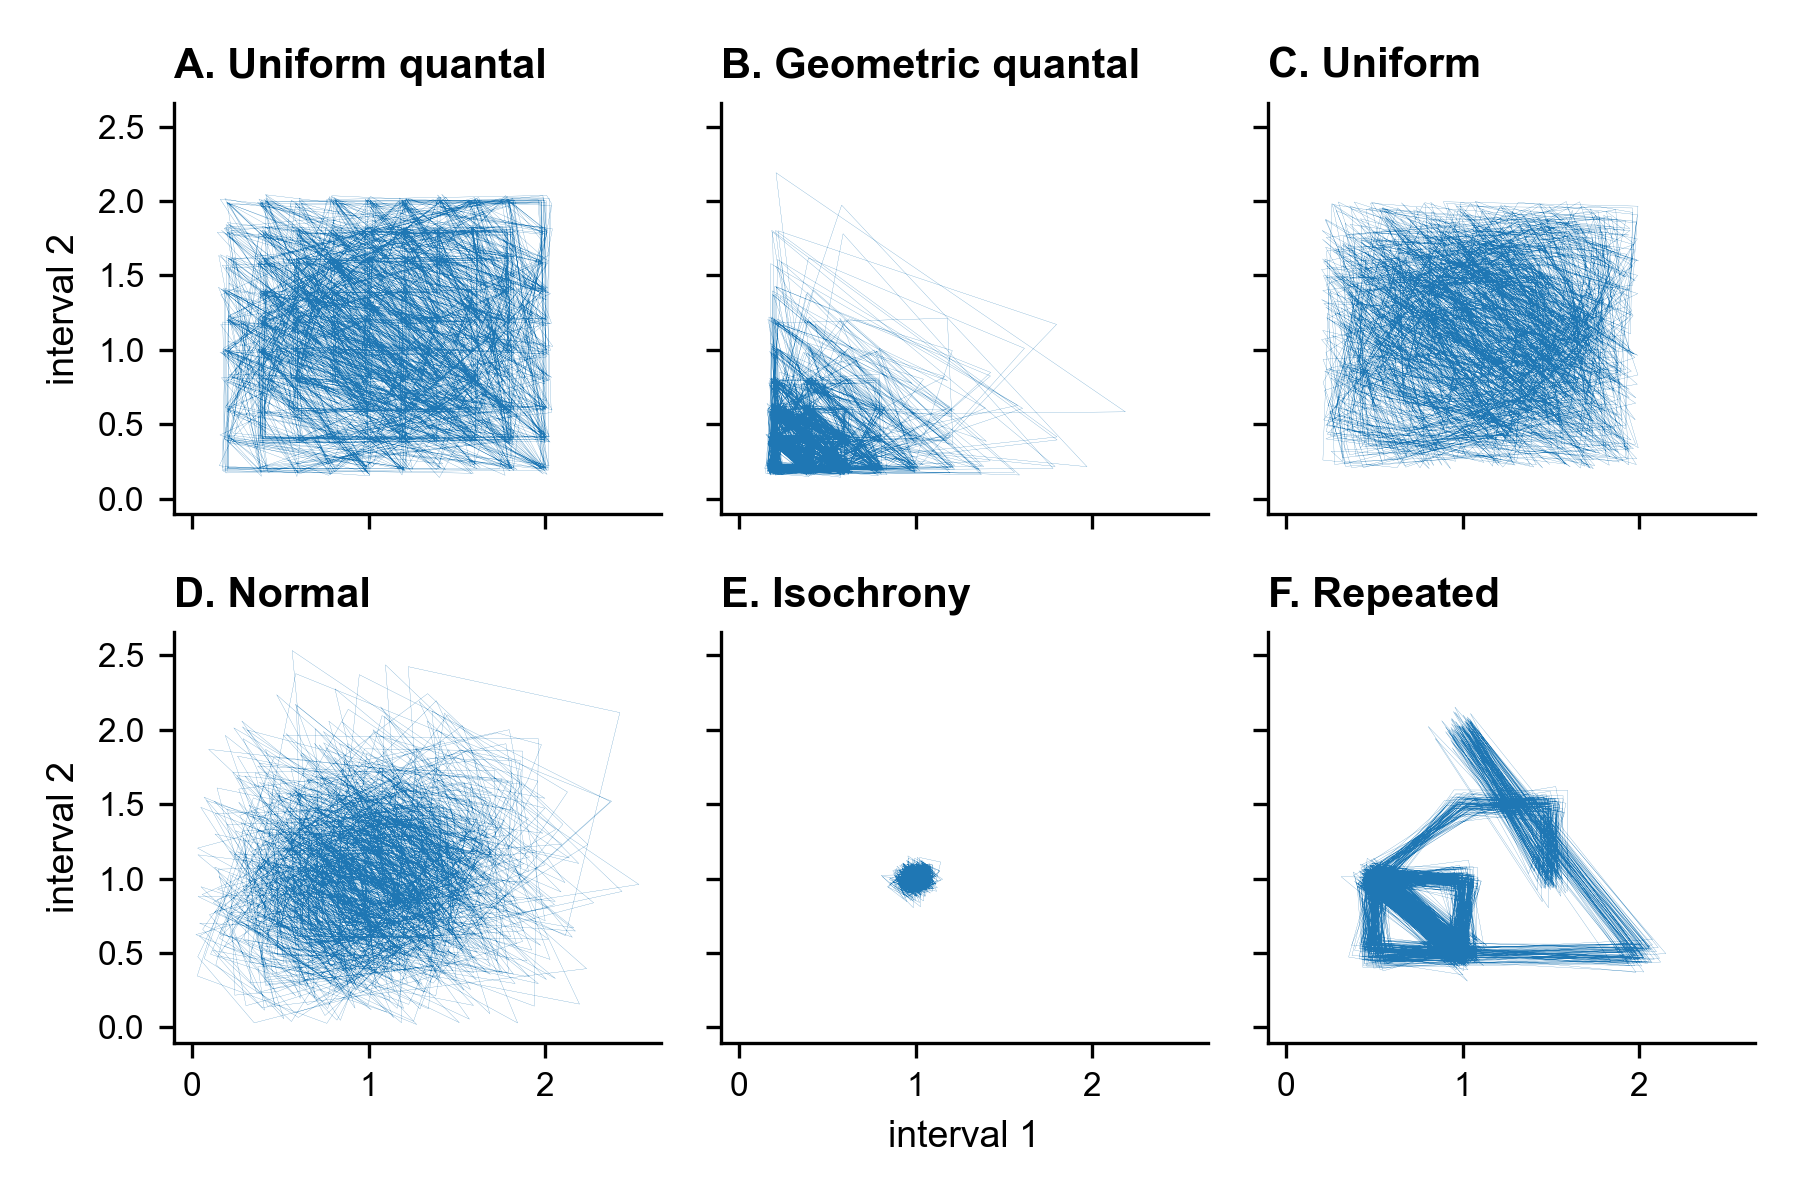
\includegraphics[width=.7\textwidth]{../../figures/plot-types/phase-plots-trajectory.png}
  \caption{
    Line phase plots of synthetic rhythmic data. 
    Similar to Figure~\ref{fig:phase-plot-scatter}, but now with a trajectory connecting successive segments. 
    The trajectory can obfuscate the clustering structure, but in data with recurrent regularities it produces distinct geometric shapes (e.g. subfigure F).
    \label{fig:phase-plot-trajectory}%
  }
\end{figure}


\begin{figure}[h!]\centering
  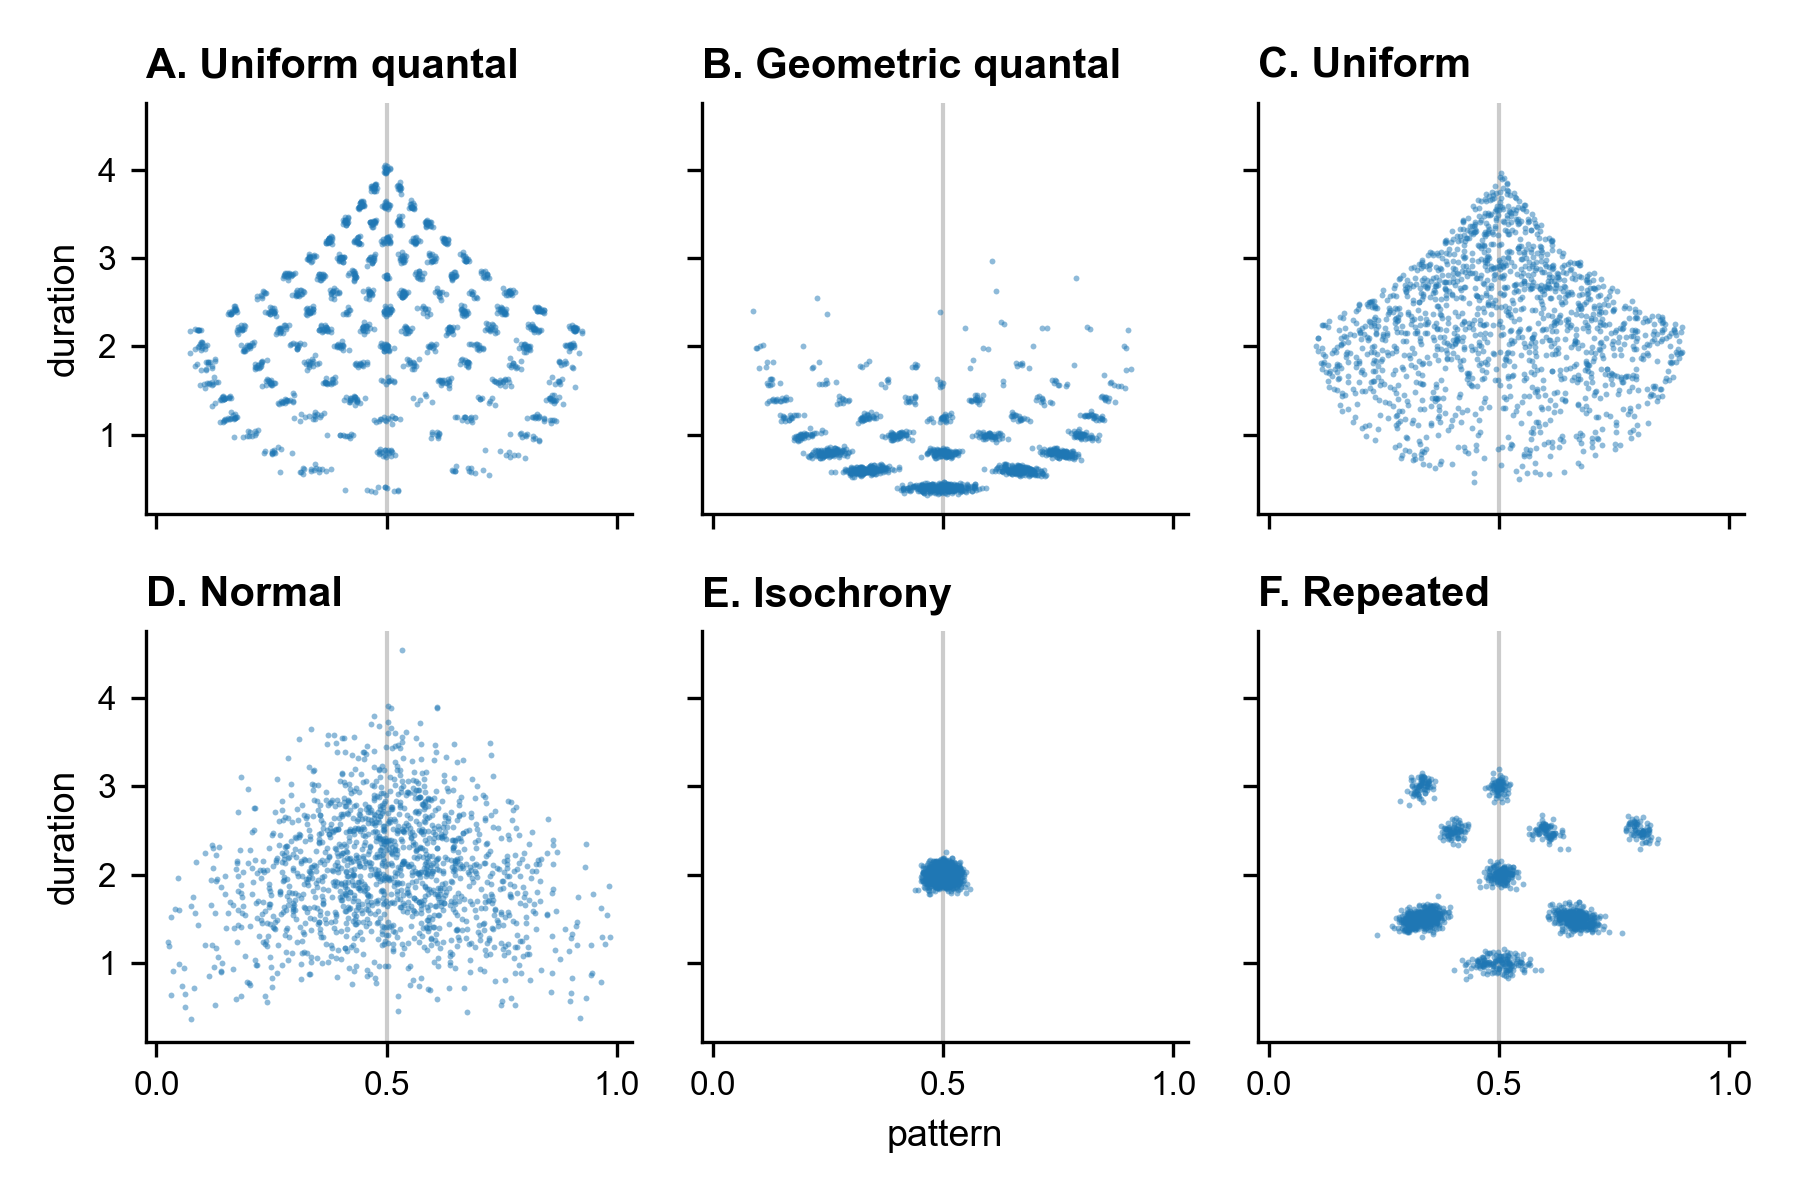
\includegraphics[width=.7\textwidth]{../../figures/plot-types/pattern-duration.png}
  \caption{%
    Pattern-duration plots for synthetic rhythmic data.
    \label{fig:pattern-duration}%
  }
\end{figure}


\begin{figure}[h!]\centering
  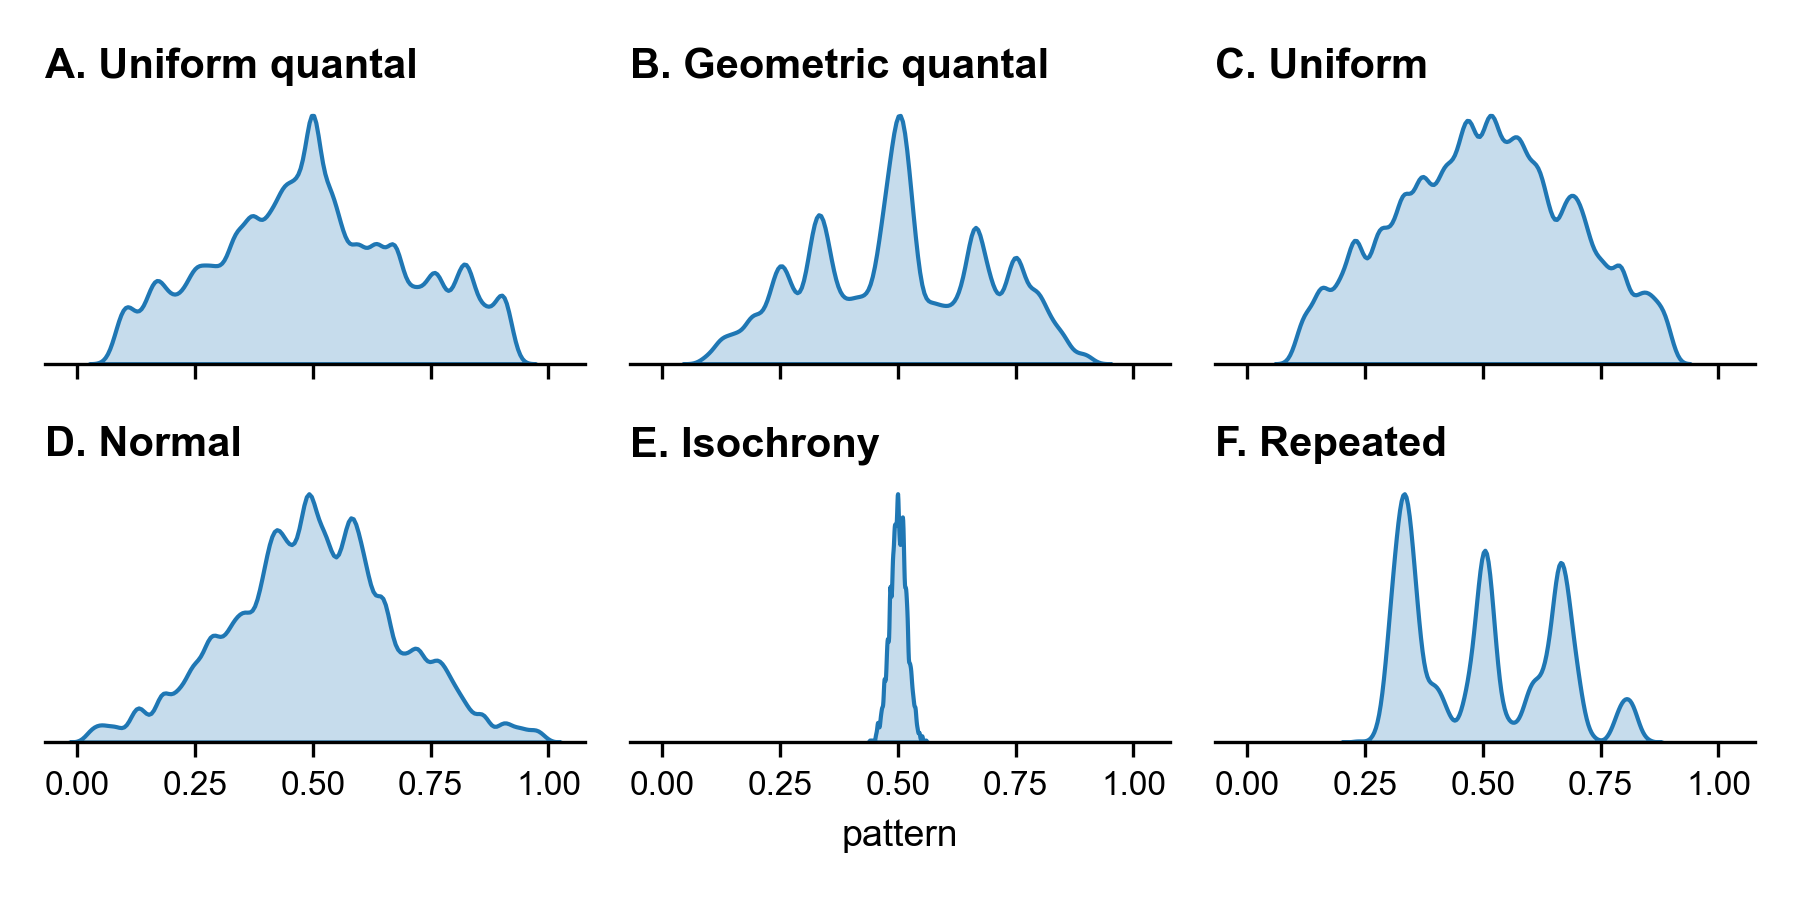
\includegraphics[width=.7\textwidth]{../../figures/plot-types/ratio-plots.png}
  \caption{%
    Ratio plots for synthetic rhythmic data.
    \label{fig:ratio-plot}%
  }
\end{figure}


\clearpage
\section{Cuban salsa and son}

% \paragraph{Cycle durations}
The main text shows pattern-duration plots of four instruments from the IEMP Cuban salsa and son (IEMP-CSS) corpus.
The metrical cycles of have been annotated and allow us to work out the 16th note duration; the cycle distribution is shown in Figure~\ref{fig:iemp-css-meter}.

% \paragraph{Pattern-duration plots per instrument}
Pattern duration plots of all instruments in song 1 are shown in Figure~\ref{fig:iemp-css-song1}. 
Plots for instruments in other songs can be found in the repository alongside the notebooks used to generate them.


\begin{figure} \centering
  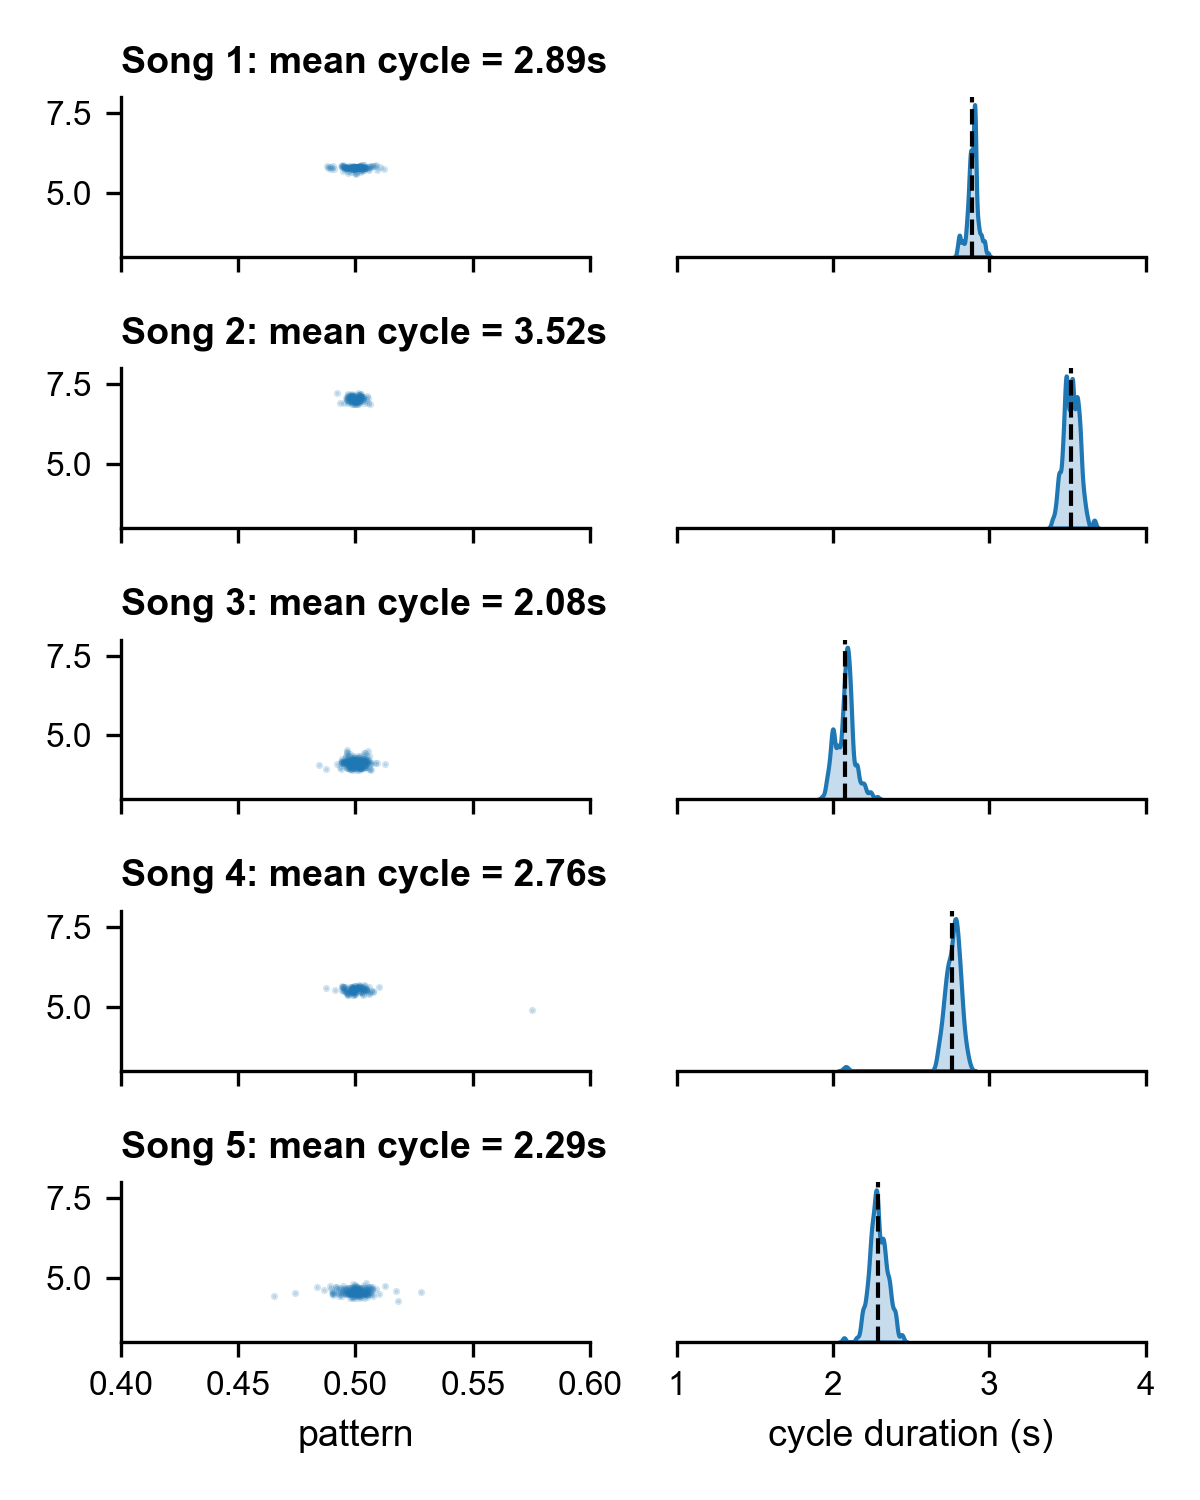
\includegraphics[width=.5\textwidth]{../../figures/iemp-css/metrical-cycles.png}
  \caption{%
    Metrical cycle duration for all of the songs in the IEMP-CSS corpus.
    Pattern-duration plots are shown on the left; the interval distribution on the right.
    \label{fig:iemp-css-meter}
  }
\end{figure}


\begin{figure}\centering
  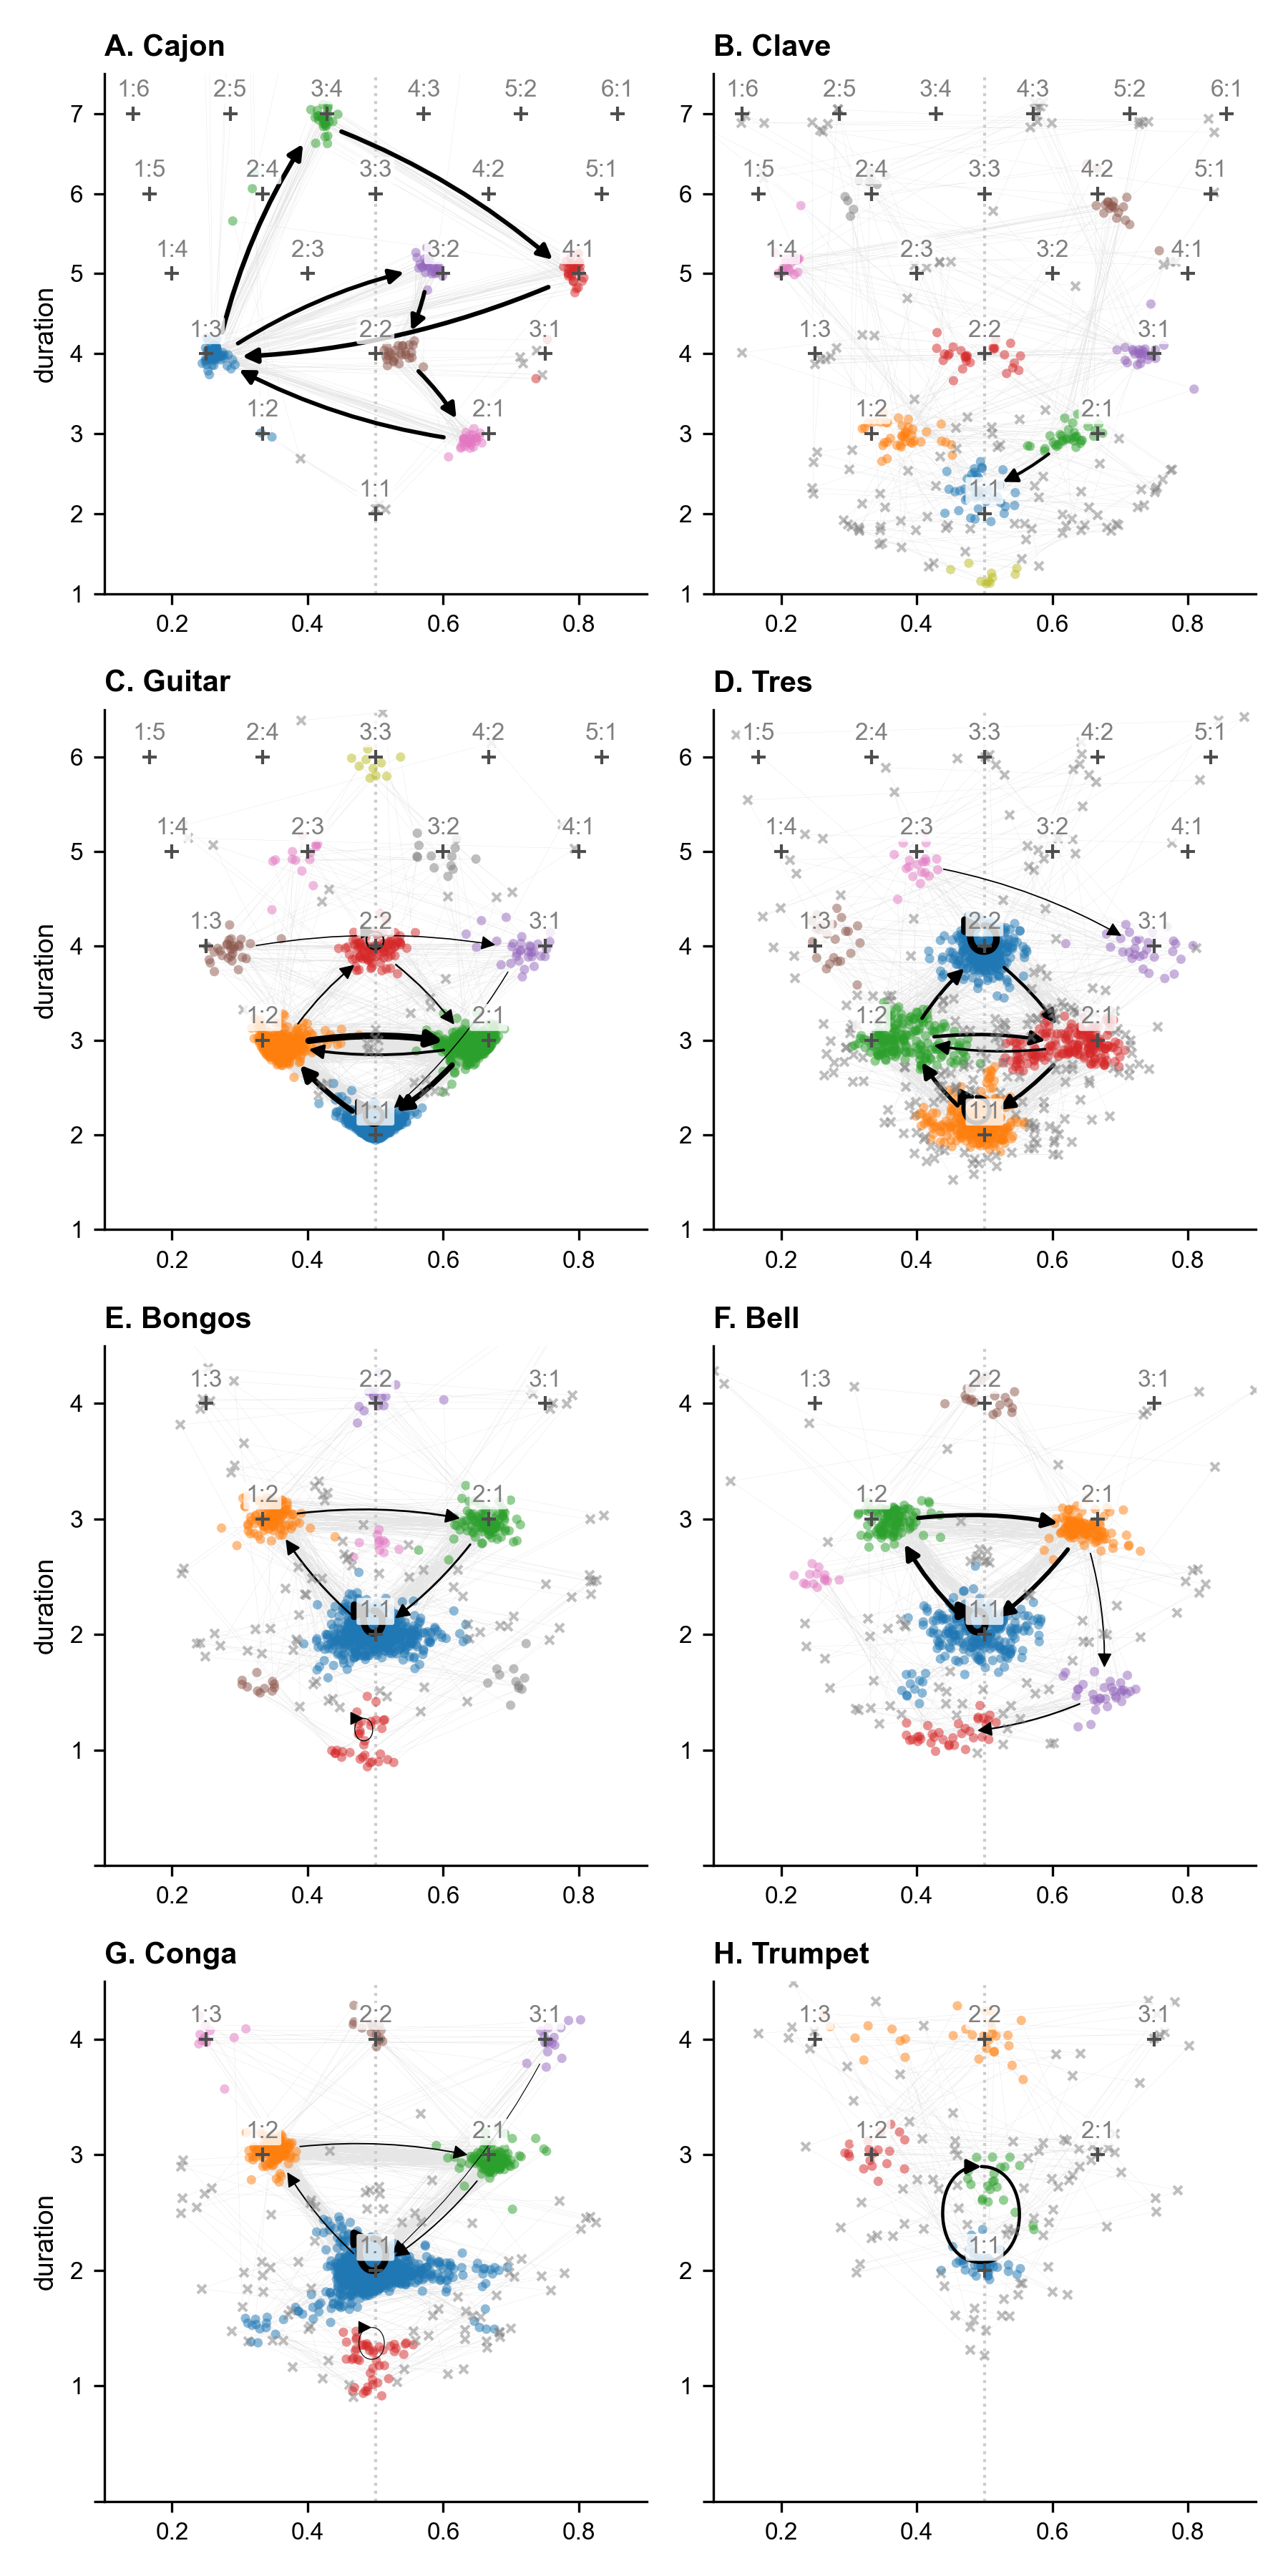
\includegraphics[height=.95\textheight]{../../figures/iemp-css/song-1-instruments.png}
  \caption{%
    Pattern-duration plots of all instruments in song 1. 
    See main text for details.
    \label{fig:iemp-css-song1}
  }


\end{figure}

\end{document}
